\subsection{Question 1}
\begin{figure}[H]
  \centering
  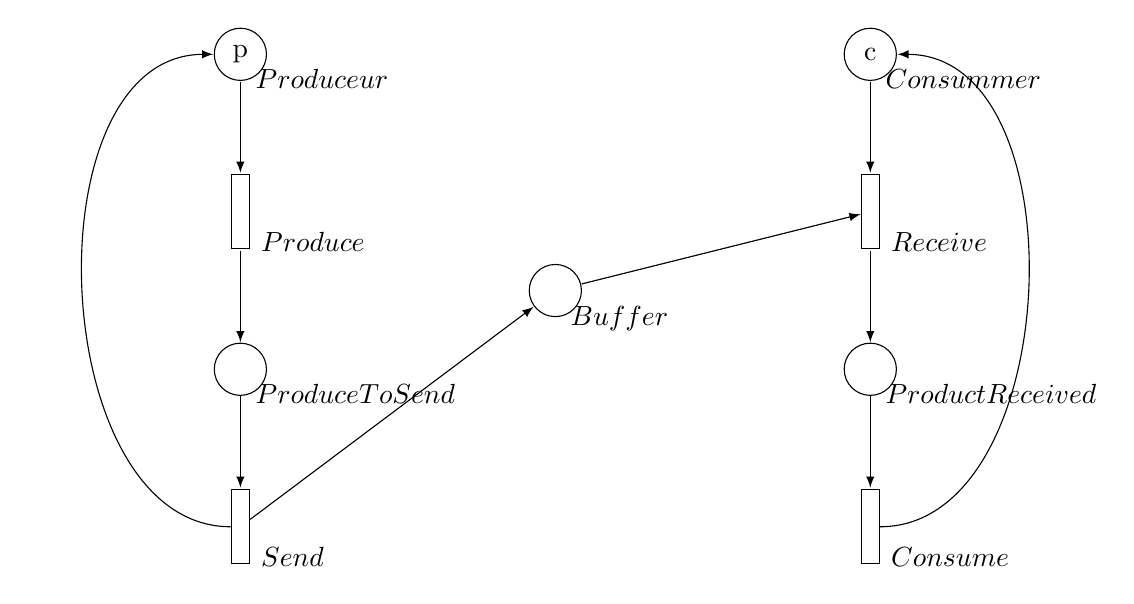
\begin{tikzpicture}

  	% Liste des places
    \draw (-4,3) node[below right = 2pt] {$Produceur$};
    \node[draw,circle,scale=2] (P) at (-4, 3) {};
    \draw (4,3) node[below right = 2pt] {$Consummer$};
    \node[draw,circle,scale=2] (C) at (4, 3) {};
    \draw (-4,-1) node[below right = 2pt] {$ProduceToSend$};
    \node[draw,circle,scale=2] (PtS) at (-4,-1) {};
    \draw (4,-1) node[below right = 2pt] {$ProductReceived$};
    \node[draw,circle,scale=2] (PR) at (4, -1) {}; %%
    \draw (0,0) node[below right = 2pt] {$Buffer$};
    \node[draw,circle,scale=2] (B) at (0, 0) {}; %%


     % Liste des transitions
    \draw (-4,1) node[below right = 4pt] {$Produce$};
    \node[draw,rectangle,yscale=4] (TP) at (-4, 1) {};
    \draw (-4,-3) node[below right = 4pt] {$Send$};
    \node[draw,rectangle,yscale=4] (TS) at (-4, -3) {};
    \draw (4,1) node[below right= 4pt] {$Receive$};
    \node[draw,rectangle,yscale=4] (TR) at (4, 1) {};
    \draw (4,-3) node[below right = 4pt] {$Consume$};
    \node[draw,rectangle,yscale=4] (TC) at (4, -3) {};

     % Liste des arcs
    \draw[->,>=latex] (P) -- (TP);
    \draw[->,>=latex] (TP) -- (PtS);
    \draw[->,>=latex] (PtS) -- (TS);
    \draw[->,>=latex] (TS) -- (B);
    \draw[->,>=latex] (B) -- (TR);
    \draw[->,>=latex] (TS) to [out=180,in=180] (P);
    \draw[->,>=latex] (C) -- (TR);
    \draw[->,>=latex] (TR) -- (PR);
    \draw[->,>=latex] (PR) -- (TC);
    \draw[->,>=latex] (TC) to [out=0,in=0] (C);

    % Marquage
    \node (p) at (-4,3) {p};
    \node (c) at (4,3) {c};

    \end{tikzpicture}
  \caption{Réseau de petri associé à l'exercice 9.1} \label{fig:M5}
\end{figure}

\subsection{Question 2}
\begin{figure}[H]
  \centering
  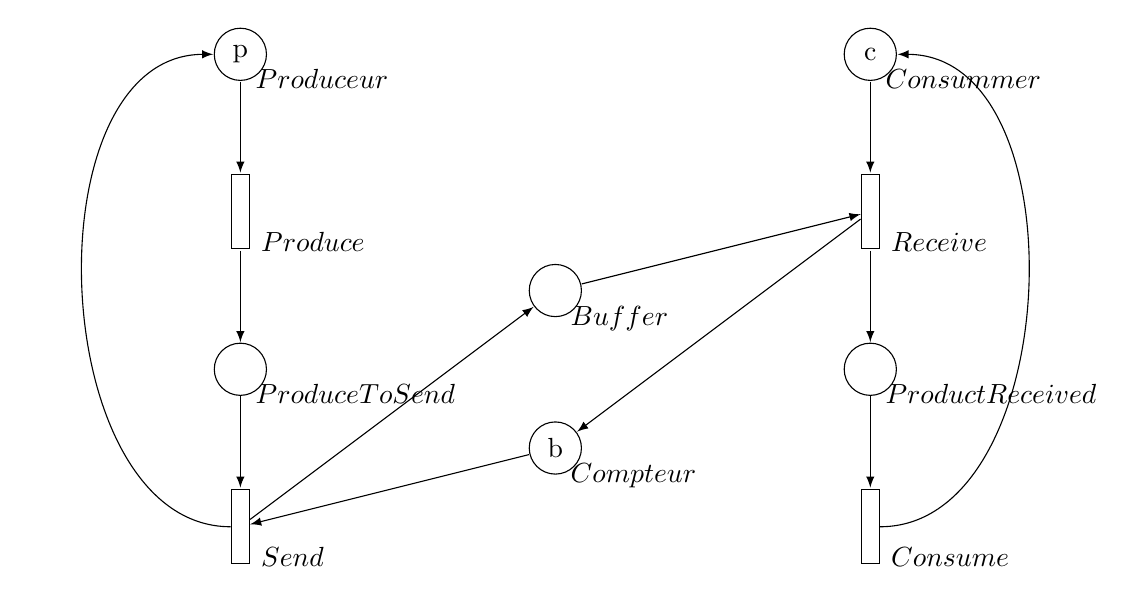
\begin{tikzpicture}

  	% Liste des places
    \draw (-4,3) node[below right = 2pt] {$Produceur$};
    \node[draw,circle,scale=2] (P) at (-4, 3) {};
    \draw (4,3) node[below right = 2pt] {$Consummer$};
    \node[draw,circle,scale=2] (C) at (4, 3) {};
    \draw (-4,-1) node[below right = 2pt] {$ProduceToSend$};
    \node[draw,circle,scale=2] (PtS) at (-4,-1) {};
    \draw (4,-1) node[below right = 2pt] {$ProductReceived$};
    \node[draw,circle,scale=2] (PR) at (4, -1) {}; 
    \draw (0,0) node[below right = 2pt] {$Buffer$};
    \node[draw,circle,scale=2] (B) at (0, 0) {}; 
    \draw (0,-2) node[below right = 2pt] {$Compteur$};
    \node[draw,circle,scale=2] (CPT) at (0, -2) {}; 


     % Liste des transitions
    \draw (-4,1) node[below right = 4pt] {$Produce$};
    \node[draw,rectangle,yscale=4] (TP) at (-4, 1) {};
    \draw (-4,-3) node[below right = 4pt] {$Send$};
    \node[draw,rectangle,yscale=4] (TS) at (-4, -3) {};
    \draw (4,1) node[below right= 4pt] {$Receive$};
    \node[draw,rectangle,yscale=4] (TR) at (4, 1) {};
    \draw (4,-3) node[below right = 4pt] {$Consume$};
    \node[draw,rectangle,yscale=4] (TC) at (4, -3) {};

     % Liste des arcs
    \draw[->,>=latex] (P) -- (TP);
    \draw[->,>=latex] (TP) -- (PtS);
    \draw[->,>=latex] (PtS) -- (TS);
    \draw[->,>=latex] (TS) -- (B);
    \draw[->,>=latex] (B) -- (TR);
    \draw[->,>=latex] (TS) to [out=180,in=180] (P);
    \draw[->,>=latex] (C) -- (TR);
    \draw[->,>=latex] (TR) -- (PR);
    \draw[->,>=latex] (PR) -- (TC);
    \draw[->,>=latex] (TC) to [out=0,in=0] (C);
    \draw[->,>=latex] (TR) -- (CPT);
    \draw[->,>=latex] (CPT) -- (TS);

    % Marquage
    \node (p) at (-4,3) {p};
    \node (c) at (4,3) {c};
    \node (b) at (0,-2) {b};

    \end{tikzpicture}
  \caption{Réseau de petri associé à l'exercice 9.2} \label{fig:M5}
\end{figure}

\subsection{Question 3}
\begin{figure}[H]
  \centering
  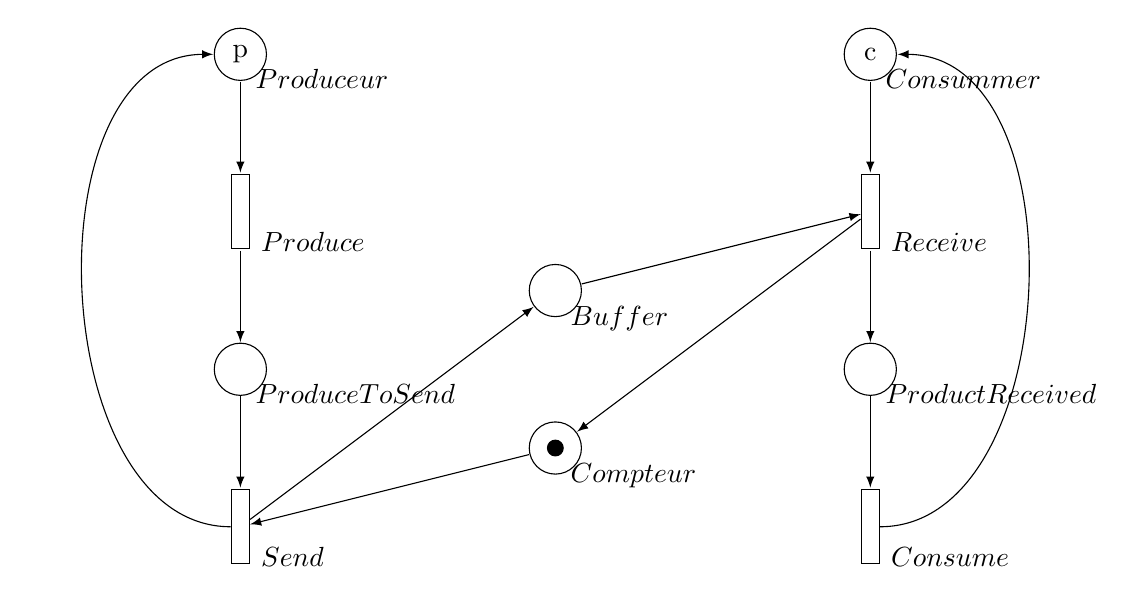
\begin{tikzpicture}

  	% Liste des places
    \draw (-4,3) node[below right = 2pt] {$Produceur$};
    \node[draw,circle,scale=2] (P) at (-4, 3) {};
    \draw (4,3) node[below right = 2pt] {$Consummer$};
    \node[draw,circle,scale=2] (C) at (4, 3) {};
    \draw (-4,-1) node[below right = 2pt] {$ProduceToSend$};
    \node[draw,circle,scale=2] (PtS) at (-4,-1) {};
    \draw (4,-1) node[below right = 2pt] {$ProductReceived$};
    \node[draw,circle,scale=2] (PR) at (4, -1) {}; 
    \draw (0,0) node[below right = 2pt] {$Buffer$};
    \node[draw,circle,scale=2] (B) at (0, 0) {}; 
    \draw (0,-2) node[below right = 2pt] {$Compteur$};
    \node[draw,circle,scale=2] (CPT) at (0, -2) {}; 


     % Liste des transitions
    \draw (-4,1) node[below right = 4pt] {$Produce$};
    \node[draw,rectangle,yscale=4] (TP) at (-4, 1) {};
    \draw (-4,-3) node[below right = 4pt] {$Send$};
    \node[draw,rectangle,yscale=4] (TS) at (-4, -3) {};
    \draw (4,1) node[below right= 4pt] {$Receive$};
    \node[draw,rectangle,yscale=4] (TR) at (4, 1) {};
    \draw (4,-3) node[below right = 4pt] {$Consume$};
    \node[draw,rectangle,yscale=4] (TC) at (4, -3) {};

     % Liste des arcs
    \draw[->,>=latex] (P) -- (TP);
    \draw[->,>=latex] (TP) -- (PtS);
    \draw[->,>=latex] (PtS) -- (TS);
    \draw[->,>=latex] (TS) -- (B);
    \draw[->,>=latex] (B) -- (TR);
    \draw[->,>=latex] (TS) to [out=180,in=180] (P);
    \draw[->,>=latex] (C) -- (TR);
    \draw[->,>=latex] (TR) -- (PR);
    \draw[->,>=latex] (PR) -- (TC);
    \draw[->,>=latex] (TC) to [out=0,in=0] (C);
    \draw[->,>=latex] (TR) -- (CPT);
    \draw[->,>=latex] (CPT) -- (TS);

    % Marquage
    \node (p) at (-4,3) {p};
    \node (c) at (4,3) {c};
    \draw [fill](0,-2) circle (0.1);

    \end{tikzpicture}
  \caption{Réseau de petri associé à l'exercice 9.3} \label{fig:M5}
\end{figure}